% apendice_b.tex: Apêndice B: Representações Visuais das Políticas Avaliadas

\chapter{Representações Visuais das Políticas Avaliadas}
\label{ap:representacoes_politicas}
\lhead{APÊNDICE B}

Este apêndice reúne representações visuais complementares das políticas avaliadas no portfólio experimental. As figuras têm caráter explicativo e servem para detalhar a lógica operacional de políticas clássicas, meta-heurísticas, agentes de aprendizado por reforço e políticas híbridas, sem alterar a formulação metodológica apresentada no Capítulo~\ref{cap:metod}. As representações incluem EOQ (Figura~\ref{fig:ap_eoq}), $(s,S)$ (Figura~\ref{fig:ap_ss}), Jornaleiro (Figura~\ref{fig:ap_jornaleiro}), Algoritmo Genético (Figura~\ref{fig:ap_ga_cromossomo}), PSO (Figura~\ref{fig:ap_pso}), Evolução Diferencial (Figura~\ref{fig:ap_de}), DQN (Figura~\ref{fig:ap_dqn}), SARSA (Figura~\ref{fig:ap_sarsa}), PPO (Figura~\ref{fig:ap_ppo}), GA-DQN (Figura~\ref{fig:ap_ga_dqn}) e GA-PPO (Figura~\ref{fig:ap_ga_ppo}).

A organização deste apêndice acompanha as famílias de métodos avaliadas na dissertação. Primeiro são apresentadas políticas clássicas, em seguida meta-heurísticas, depois agentes de aprendizado por reforço e, por fim, uma representação complementar de política híbrida GA-RL.

\begin{figure}[htbp]
    \centering
    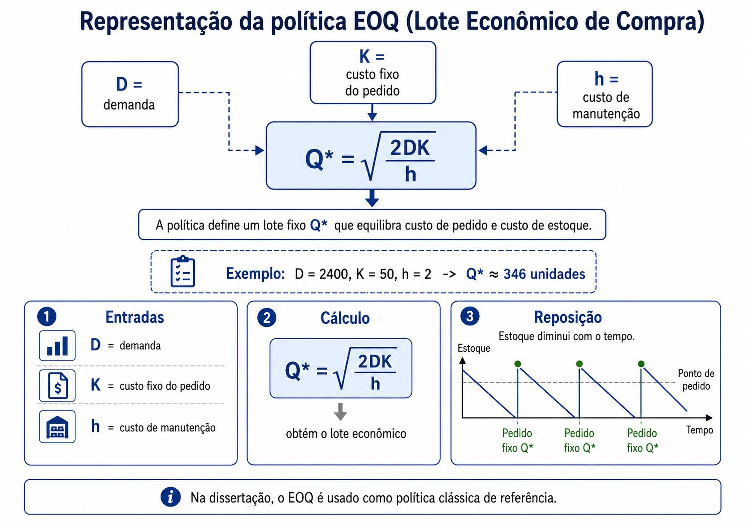
\includegraphics[width=0.86\textwidth]{img/política_eoq_lote_econômico_de_compra.pdf}
    \caption{Representação da lógica do lote econômico de compra (EOQ).}
    \label{fig:ap_eoq}
\end{figure}

Enquanto o EOQ enfatiza o equilíbrio entre custo de pedido e custo de manutenção, a política $(s,S)$ explicita uma regra operacional de revisão: quando a posição de estoque atinge o ponto de reposição \(s\), emite-se pedido para recompor o nível-alvo \(S\). A Figura~\ref{fig:ap_ss} resume essa lógica.

\begin{figure}[htbp]
    \centering
    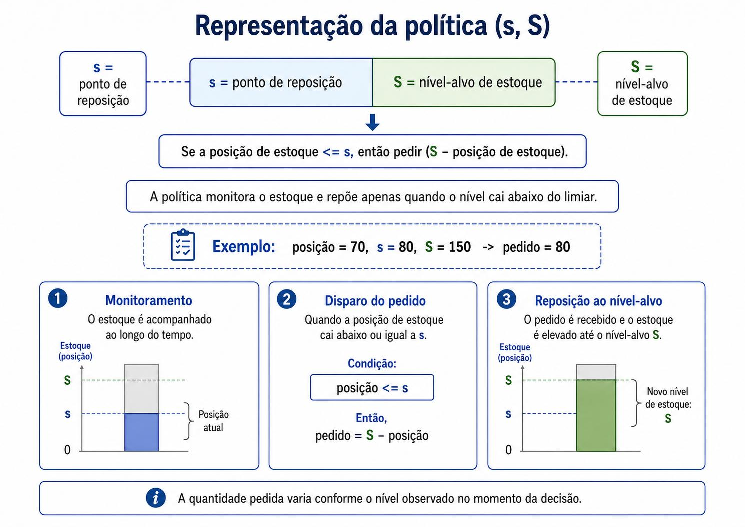
\includegraphics[width=0.86\textwidth]{img/política_de_reposição_de_estoques.pdf}
    \caption{Representação conceitual da política $(s,S)$ no controle de inventário.}
    \label{fig:ap_ss}
\end{figure}

A política do jornaleiro considera explicitamente o equilíbrio entre risco de excesso e risco de falta. Essa diferença motiva sua inclusão como referência clássica no portfólio experimental.

\begin{figure}[htbp]
    \centering
    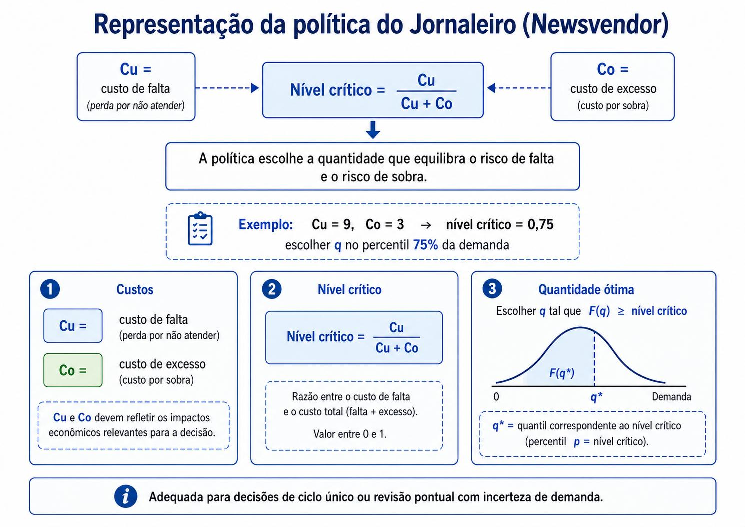
\includegraphics[width=0.86\textwidth]{img/política_do_jornaleiro_infográfico_explicativo.pdf}
    \caption{Representação da política do jornaleiro para decisão de reposição sob incerteza de demanda.}
    \label{fig:ap_jornaleiro}
\end{figure}

As meta-heurísticas avaliadas usam representações contínuas para buscar parâmetros de reposição com bom desempenho operacional. No Algoritmo Genético, cada cromossomo codifica uma parametrização candidata da política de reposição, como mostra a Figura~\ref{fig:ap_ga_cromossomo}.

\begin{figure}[htbp]
    \centering
    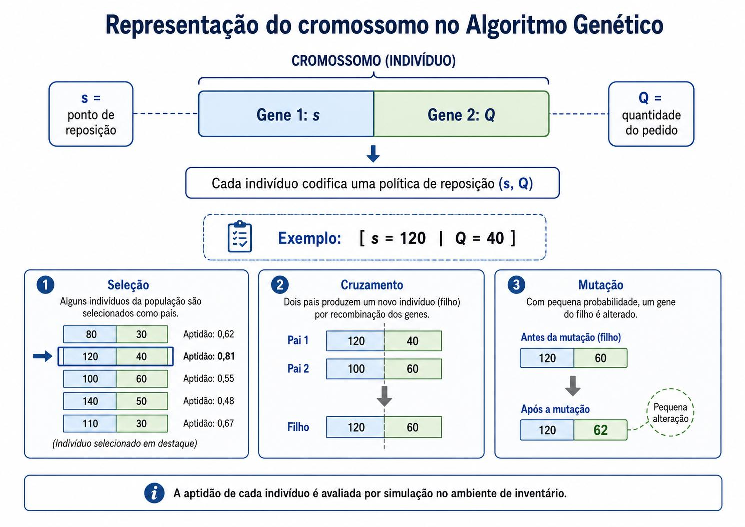
\includegraphics[width=0.86\textwidth]{img/representação_do_cromossomo_no_ag.pdf}
    \caption{Representação do cromossomo no Algoritmo Genético para parametrização de políticas de reposição.}
    \label{fig:ap_ga_cromossomo}
\end{figure}

A Figura~\ref{fig:ap_pso} apresenta a representação complementar do PSO, em que cada partícula corresponde a uma solução candidata no espaço de busca.

\begin{figure}[htbp]
    \centering
    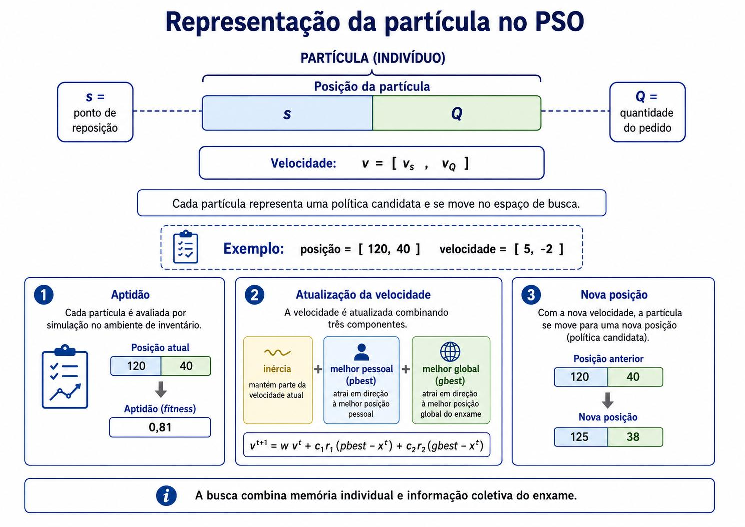
\includegraphics[width=0.86\textwidth]{img/representação_da_partícula_no_pso.pdf}
    \caption{Representação de uma partícula no Particle Swarm Optimization aplicada à parametrização de políticas de reposição.}
    \label{fig:ap_pso}
\end{figure}

Diferentemente do PSO, que atualiza partículas a partir de memória individual e coletiva, a Evolução Diferencial gera novos candidatos por combinações diferenciais entre vetores da população. Ambas as abordagens são usadas como mecanismos de busca em espaços contínuos de parametrização.

\begin{figure}[htbp]
    \centering
    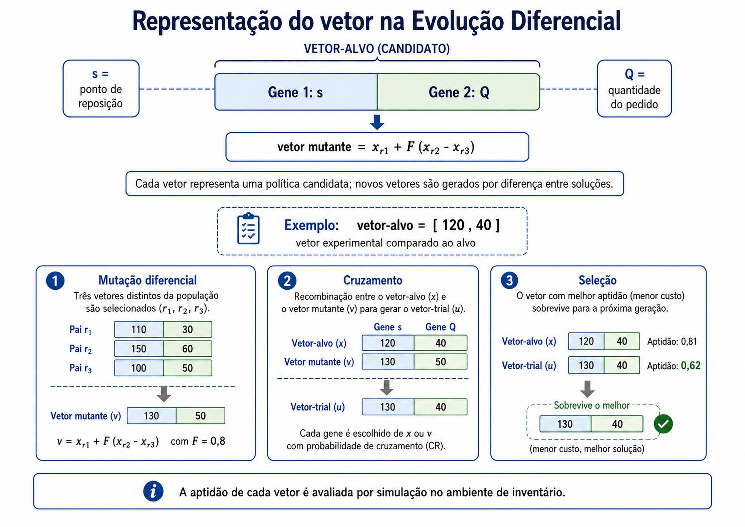
\includegraphics[width=0.86\textwidth]{img/representação_do_vetor_na_evolução_diferencial.pdf}
    \caption{Representação de um vetor-solução na Evolução Diferencial aplicada ao problema de reposição.}
    \label{fig:ap_de}
\end{figure}

Nos agentes de aprendizado por reforço, a decisão de reposição é tratada como interação sequencial entre agente e ambiente. A Figura~\ref{fig:ap_dqn} resume a lógica do DQN, no qual o estado observado é usado para estimar valores associados a ações candidatas de reposição.

\begin{figure}[htbp]
    \centering
    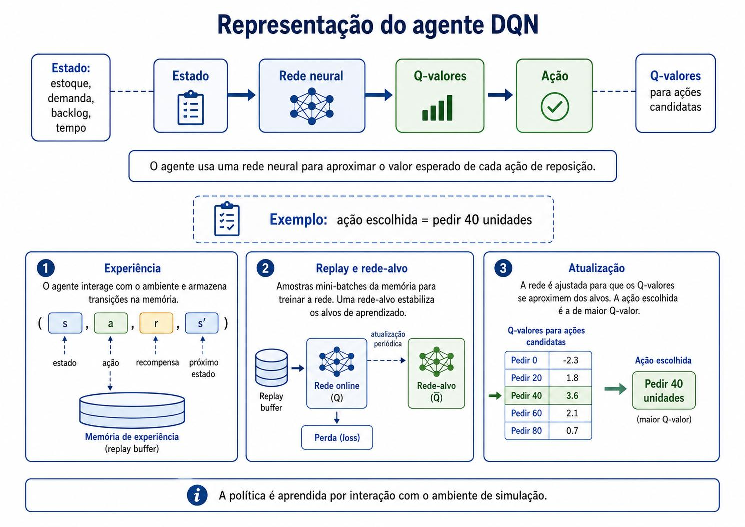
\includegraphics[width=0.86\textwidth]{img/representação_do_agente_dqn.pdf}
    \caption{Representação do agente Deep Q-Network (DQN) no ambiente de reposição.}
    \label{fig:ap_dqn}
\end{figure}

A Figura~\ref{fig:ap_sarsa} detalha a estrutura do SARSA, que atualiza sua política com base na trajetória efetivamente seguida.

\begin{figure}[htbp]
    \centering
    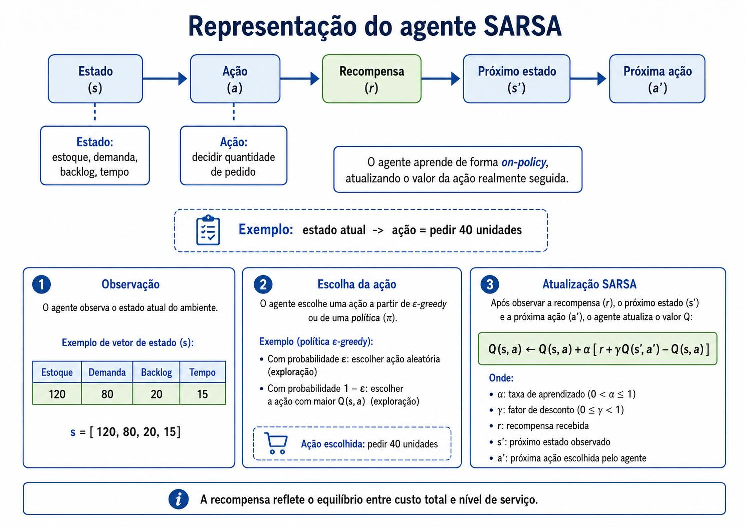
\includegraphics[width=0.86\textwidth]{img/representação_do_agente_sarsa_detalhada.pdf}
    \caption{Representação do agente SARSA no problema de controle de inventário.}
    \label{fig:ap_sarsa}
\end{figure}

Na política \(\epsilon\)-greedy, a escolha aleatória de uma ação corresponde à etapa de exploração, enquanto a seleção da ação com maior valor \(Q(s,a)\) corresponde ao aproveitamento da melhor ação estimada. Essa distinção é importante para interpretar corretamente o mecanismo de escolha de ações no agente SARSA.

Os agentes SARSA e PPO compartilham a abstração de interação sequencial com o ambiente, mas diferem na forma de atualização da política. Enquanto o SARSA atualiza valores de ação de forma \textit{on-policy}, o PPO utiliza uma estrutura ator-crítico com atualização controlada da política.

\begin{figure}[htbp]
    \centering
    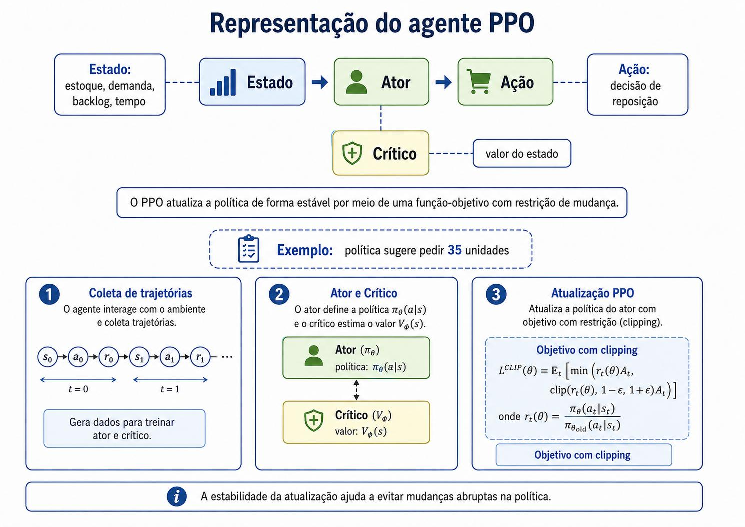
\includegraphics[width=0.86\textwidth]{img/representação_do_agente_ppo_em_detalhes.pdf}
    \caption{Representação do agente Proximal Policy Optimization (PPO) aplicado ao controle de inventário.}
    \label{fig:ap_ppo}
\end{figure}

Por fim, as políticas híbridas GA-DQN e GA-PPO complementam a família GA-RL ao combinar busca evolutiva com refinamento por aprendizado por reforço. A Figura~\ref{fig:ap_ga_dqn} ilustra a lógica de inicialização evolutiva e refinamento por DQN.

\begin{figure}[htbp]
    \centering
    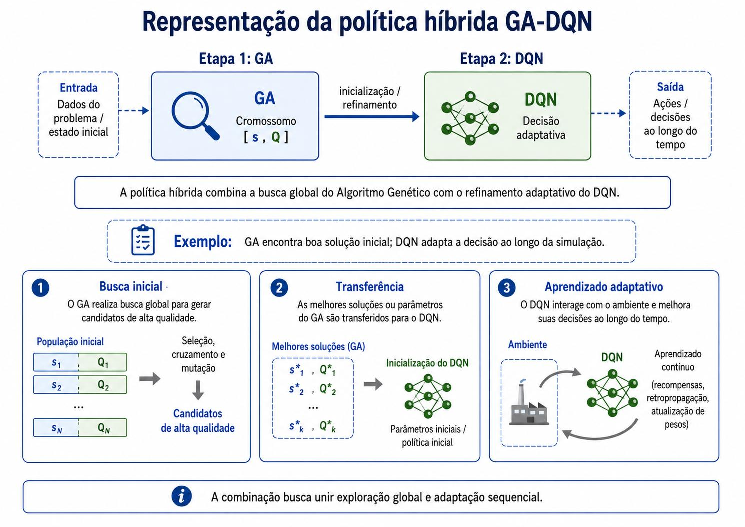
\includegraphics[width=0.86\textwidth]{img/representação_da_política_híbrida_ga_dqn.pdf}
    \caption{Representação da política híbrida GA-DQN no portfólio avaliado.}
    \label{fig:ap_ga_dqn}
\end{figure}

A Figura~\ref{fig:ap_ga_ppo} apresenta a variante GA-PPO. Essa representação reforça que as políticas híbridas são tratadas como especialistas do portfólio avaliado, mantendo o AIPE e o PSE como contribuição metodológica central.

\begin{figure}[htbp]
    \centering
    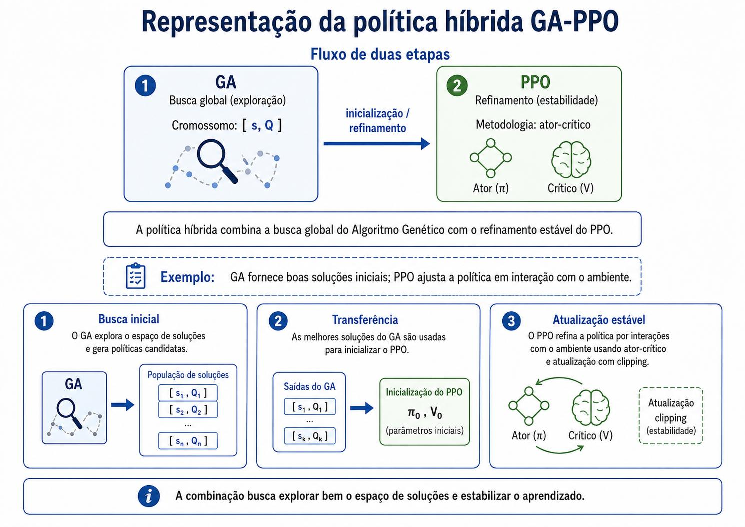
\includegraphics[width=0.86\textwidth]{img/fluxo_da_política_híbrida_ga_ppo.pdf}
    \caption{Fluxo da política híbrida GA-PPO no contexto do controle de inventário.}
    \label{fig:ap_ga_ppo}
\end{figure}
